\section{The Bias and Mean Square Error of Point Estimators}
A start at trying to determine if a point estimator is any good.

\nl Let $\that$ be a point estimator for a parameter $\theta$. (e.g. $\theta = \mu, \quad \that = \Xbar$)
\begin{enumerate}[label=\textcircled{\raisebox{-1pt}{\arabic*}}]
    \item 
        One goal of a good estimator is that $E(\that) = \theta$ (e.g. by CLT, $\E{\Xbar} = \mu$)\\But this is not always the case.
        
        \defn If $\Eb*{\that}=\theta$, we say that $\that$ is an \textbf{\underline{unbiased}} point estimator.\\(e.g. $\Xbar$ is unbiased).

        \nl If $\that$ is a biased point estimator, we define the \underline{\textbf{bias}} to be
        $$\bias*{\that} = \Eb*{\that} - \theta$$
    
    \item 
        Another goal of a good estimator might be that its \say{spread} of observations is tightly packed (talking about variance), and hopefully near $\theta$.
        $$\text{spread}\, \Longrightarrow \text{variance}$$
        \defn* The \textbf{\underline{mean square error}} of $\that$ is
        $$MSE(\that) = E\brac{(\that - \theta)^2}$$
        Recall: $V[X] = E[X^2] - (E[X])^2$
        
        \nl \textbf{Corollary:}
        $$\MSE*{\that} = \Var*{\that} + \bigbrac{\bias*{\that}}^2$$
        \begin{proof}
            \begin{align*}
                \MSE*{\that} &= \Eb*{\that^2 - 2\that \theta + \theta ^2}\\
                &= \Eb*{\that^2} - 2\Eb*{\that\theta} + \Eb*{\theta ^2} \\
                &= \blue{\Eb*{\that^2}} - 2\Eb*{\that}\theta + \theta^2 \\
                &= \blue{\Eb*{\that^2} - \pars*{\Eb*{\that}}^2 + \pars*{\Eb*{\that}}^2} - 2\Eb*{\that}\theta + \theta ^2\\
                &= \Var*{\that} + \pars*{\Eb*{\that}-\theta}^2\\
                &= \Var*{\that} + \pars*{\bias*{\that}}^2
            \end{align*}
        \end{proof}
\remark We have decomposed MSE by:
$$\MSE*{\that} = \underbrace{\Var*{\that}}_{\text{Precision}} + \underbrace{\bias*{\that}^2}_{\text{Accuracy}}$$
\end{enumerate}
Idea of a \say{best} estimator is tricky. We'd like MSE to be as small as possible, but this is an impossible problem because MSE depends on the unknown $\that$.

\example (Population proportions). Want $p$.

\nnl To estimate, let
$$Y = \begin{cases} 
      1 & \text{\say{success}} \\
      0 & \text{\say{failure}} 
   \end{cases}$$
and $\{Y_i\}$ be an iid random sample.

\nnl \textbf{\red{Estimator 1:}} $\displaystyle \phat = \over{n}\sum Y_i = \Ybar$

\nl This sums the $\frac{\text{people said yes}}{\text{total people}}$

\recall* $\sum Y_i$ is $\text{binom}(n,p)$.

\nnl And for a Binomial Distribution, we know
$$\Eb{X} = np \wideand \Var{X} = npq = np(1-p)$$
Bias? Then what is the $\Eb*{\phat}$?
$$\Eb*{\phat} = \E{\over{n}\sum Y_i} = \over{n}\E{\sum Y_i} = \over{n}\cdot np = p$$
Because $\Eb*{\phat} = p$, then $\phat$ is an \underline{unbiased} estimator. For $\MSE*{\phat}$, we need $\Varb*{\phat}$:
$$\Varb*{\phat} = \Var{\over{n}\sum Y_i} = \pover{n}^2 \Var{\sum Y_i} = \pars{\over{n}}^2 np(1-p) = \frac{p(1-p)}{n}$$
Therefore,
\begin{align*}
    \MSE*{\phat} &= \Var*{\phat} - \bias*{\phat}^2\\
    &= \frac{p(1-p)}{n} + \underbrace{0^2}_{\text{\say{unbiased}}}
\end{align*}

\nnl \textbf{\red{Estimator 2: }} $\displaystyle \ptilde = \frac{\sum_1^n Y_i + 1}{n+2}$

$$n = 1, \qquad y = \begin{cases} 
      1\\
      0
   \end{cases} \qquad \ptilde = \begin{cases} 
      2/3 & \\
      1/3 \\
   \end{cases}$$
   $$n = 2, \qquad y = \begin{cases} 
      2\\
      1\\
      0
   \end{cases} \qquad \ptilde = \begin{cases} 
      3/4 \\
      2/4\\
      1/4
   \end{cases}$$
$$\Eb*{\ptilde} = \frac{\E{Y_i} + \E{1}}{n+2} = \frac{np+1}{n+2} = p + \frac{1-2p}{n+2} \neq p$$
Hence, $\ptilde$ is \underline{biased}. And,
$$\bias*{\ptilde} = \Eb*{\ptilde} - p = p + \frac{1-2p}{n+2} - p = \frac{1-2p}{n+2}$$

\nnl\textbf{Calc question:} What happens to $\Eb*{\ptilde}$ as sample size grows? ($\Eb*{\ptilde} \to p$)

\nnl Need
\begin{align*}
    \Var{\ptilde} &= \Var{\frac{\sum_1^n Y_i + 1}{n+2}} \\
    &=  \Var{\frac{\sum_1^n Y_i}{n+2} + \over{n+2}} \\
    &= \Var{\frac{\sum_1^n Y_i}{n+2}} \\
    &= \over{(n+2)^2} \Var{\sum_1^n Y_i} \\
    &= \frac{np(1-p)}{(n+2)^2}
\end{align*}
Then
\begin{align*}
    \MSE*{\ptilde} &= \Var{\ptilde} + \bias*{\ptilde}^2\\
    &= \frac{np(1-p)}{(n+2)^2} + \pars{\frac{1-2p}{n+2}}^2\\
    &= \frac{np(1-p) + (1-2p)^2}{(n+2)^2}
\end{align*}


\nl \textbf{Q:} Which estimator is better? \hspace{0.25in} \textbf{A:} \textit{it depends!}

\nnl Note that for both, $\MSE*{\ptilde}(n,p)$ are functions of $n$ and $p$. Let
$$\red{y=\MSE*{\ptilde}(n,p)} \wideand \blue{y=\MSE*{\phat}(n,p)}$$
\newpage
$$\text{fix } n = 10, \qquad p \in[0,1]$$
\begin{center}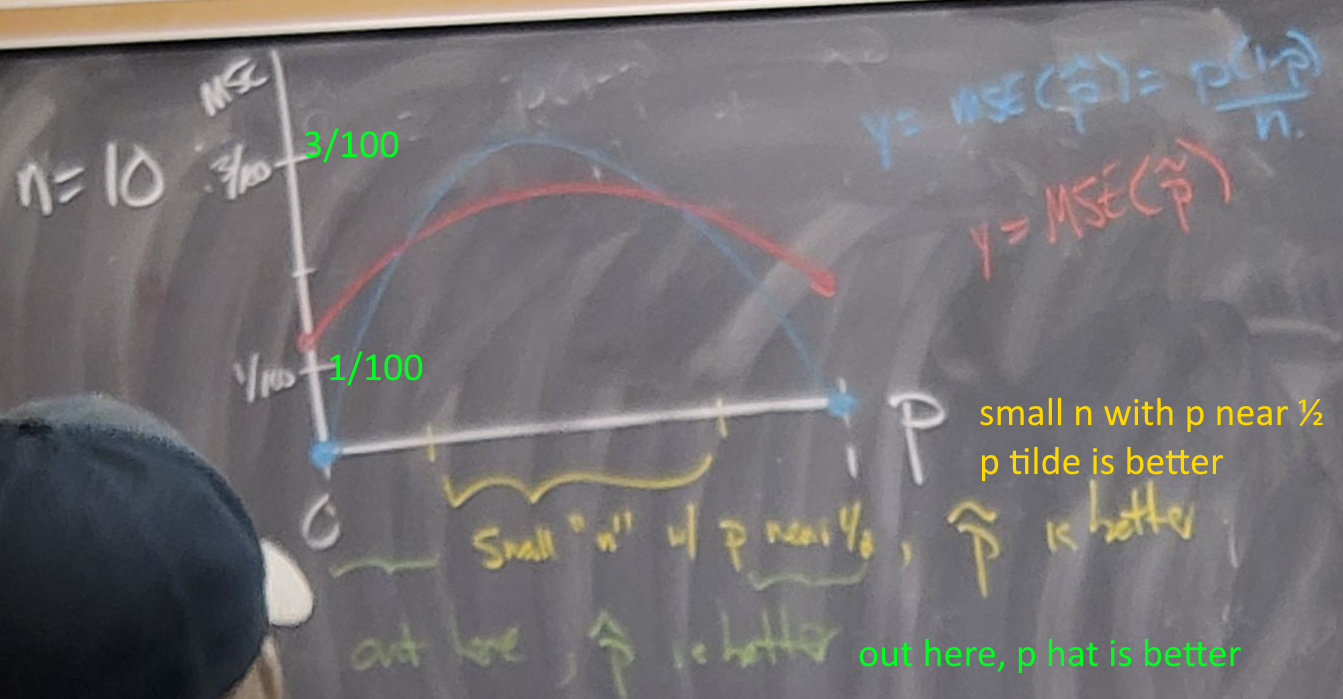
\includegraphics[width=15cm]{mse n 10.png}\end{center}

$$n = 25 \text{ and } 100 \qquad p \in [0,1]$$
\begin{center}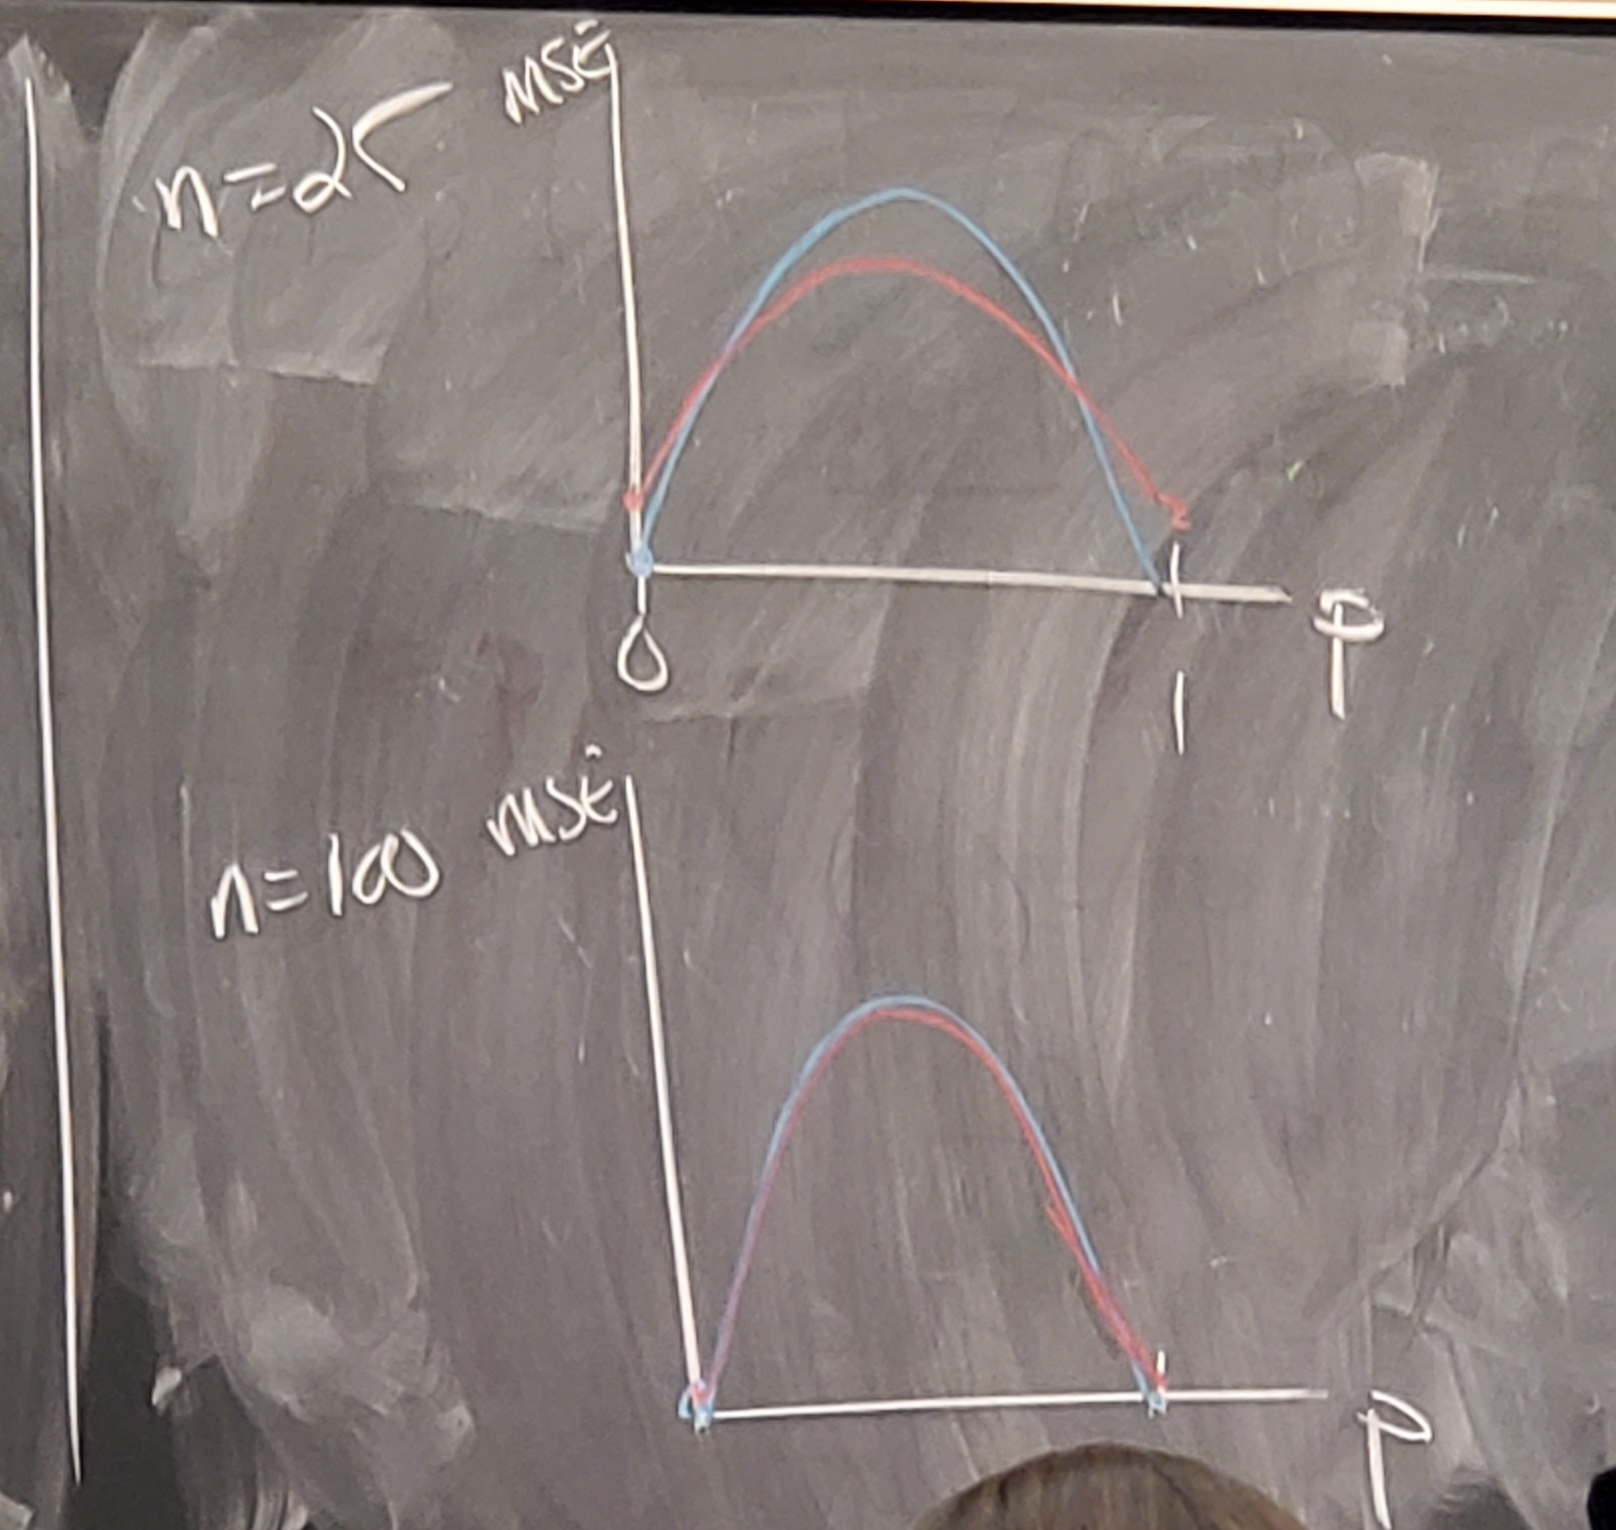
\includegraphics[width=4.5in]{mse 25 and 100.png}\end{center}
For larger $n$, they become indistinguishable.